


\begin{figure}
\setlength{\unitlength}{\textwidth}

  \begin{picture}(1,0.4)(0,0.75)
    
 \put(0.2,0.76){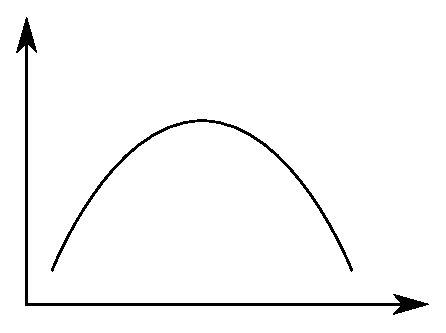
\includegraphics[width=0.5\unitlength]{../FnP/gnuplot/sketch_1.eps}}         
      
     
 	\put(0.1,0.93){$\displaystyle\frac{P_{m}}{\rho \mathcal{A}U^3 }$}
 \put(0.406,1){\ding{193}}
 \put(0.265,0.9){\ding{192}}
 \put(0.535,0.935){\ding{194}}
    \put(0.42,0.74){$\massdamp$}
    
      	

 	
 	 


  \end{picture}

 \caption{ Three key regions taken into account to analyse the time histories of power in a typical mean power vs. $U^*$ curve at $Re=200$. In region 1, high damping suppresses oscillation, hence the power output is low. In region 2, the damping is close to the optimum for power transfer. In region 3, the low damping means little energy is extracted from the fluid.}
 \label{fig:regions_1}
\end{figure}


















